\section{Implications of the methodology in the context of \glsfmtshort{WCA}}\label{sec:extendingmethodology}

\todo[inline]{%
    Rework this section.
    First, discuss that we wish a more detailed study on the implications of the methodology for the optimization of WCA.
    However, to achieve that we must first improve upon our model of human behavior.
    This leads to us first characterizing human behavior, to then building an improved model.
}

\todo[inline]{%
    Why do we need to extend the methodology? What was wrong with the approach in the previous section?
}

\subsection{Characterizing human behavior}

\cref{paper:olguinmunoz2021impact} describes a study designed to characterize the effects of system responsiveness on human behavior in step-based \gls{WCA}.
This corresponds to the first step in extending our EdgeDroid tool for the benchmarking of \gls{WCA}, first introduced in \cref{paper:olguinmunoz2018demoscaling,paper:olguinmunoz2019edgedroid}, with a more realistic model of human behavior.

We present in this paper the design and execution of a study in which \num{40} undergraduate students of diverse fields of
study\footnote{%
    Participants were recruited from a pool of students enrolled in an undergraduate psychology course at \gls{CMU}.
}, were asked to interact with and follow the instructions given to them by a \gls{WCA} application.
Unbeknownst to the participants, the system responsiveness of the \gls{WCA} system was systematically altered in real time, and the resulting behavioral and physiological reactions were recorded.

With this study, we intended to answer four core research questions relating to human responses to decreased application responsiveness.
One, do subjects change the temporal profile of their actions in relation to system latency?
We expected this to be the case, although the extent or form of these changes were unknown.
Two, do users show signals of arousal in physiological responses to changes in system latency?
As latency increased and due to the added annoyance of dealing with a less responsive system, we expected users to begin showing signs of stress and frustration.
Three, are responses to delay effects in subjects mediated by cognition and/or emotion?
We expected delay effects in subjects to be mediated primarily by emotion, and in particular expected these effects to be correlated with the level of the reduction in system responsiveness.
And four, are these effects mediated by personality indicators in any way?
It was our hypothesis that, among others, the individual trait of \emph{neuroticism}~\cite{john1999big} would play a particularly important role in mediating effects of reduced system responsiveness on subjects.

Our results partially agree with our initial hypotheses.
We found that reduced system responsiveness induces \emph{additional} behavioral slow-down in users of \gls{WCA}.
This additional slow-down moreover scales with the strength of the reduction in system responsiveness.
Furthermore, we note that humans tend to speed up as the task progresses.
However, as system responsiveness decreases, this effect is strongly dampened.
We also found that the effects of reduced system responsiveness on users linger for at least \num{4} steps after system responsiveness improves, leading to longer execution times for steps immediately after a period of reduced responsiveness.

Finally, we also found that the above effects are modulated by measures of individual levels of personality.
In particular, the trait of \emph{neuroticism} seems to play a significant role in modulating users' response to reduced responsiveness in \gls{WCA}.

\subsubsection{Methodology}

\begin{figure}[tb]
    \centering
    \begin{subfigure}[t]{.49\textwidth}
        \centering
        \includegraphics[width=\textwidth]{publications/2021ImpactDelayedResponse/Fig4a}
        \caption{}\label{sfig:regularwcaexec}
    \end{subfigure}%
    \hfill%
    \begin{subfigure}[t]{.49\textwidth}
        \centering
        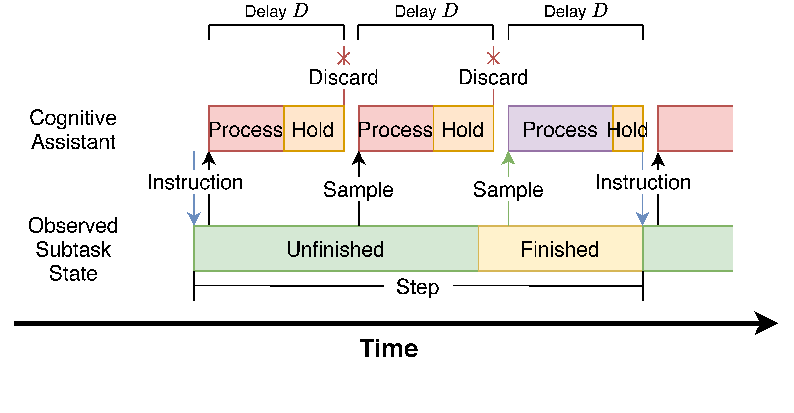
\includegraphics[width=\textwidth]{publications/2021ImpactDelayedResponse/Fig4b}
        \caption{}\label{sfig:delaywcaexec}
    \end{subfigure}
    \caption{%
        Comparison between normal task execution in the LEGO \gls{WCA}~\cite{chen2015early}~(\labelcref{sfig:regularwcaexec}) and modified task execution with delay in the experimental setup of \cref{paper:olguinmunoz2021impact}~(\labelcref{sfig:delaywcaexec}).
        In the experimental task, an additional variable segment of time is introduced immediately following the processing of the input frame in order to extend the perceived processing time of the input to a specific target interval of time denoted \emph{delay}.
    }\label{fig:regularwca-vs-delaywca}
\end{figure}

We employed a version of the step-based \emph{Gabriel} cognitive assistant framework first introduced by \citeauthor{chen2018application}~\cite{chen2018application}.
The assistant was instrumented to capture key application and task performance metrics in real time, in particular step execution time.
Furthermore, the software was modified to allow for the real-time alteration of system responsiveness by extending the processing interval of each input to a temporarily fixed value denoted \emph{delay}.
This is illustrated in \cref{fig:regularwca-vs-delaywca}.
If, during a series of steps, delay was set to a value \ensuremath{\mathbb{D}}, the feedback for each input frame was provided to the user exactly a time interval \ensuremath{\mathbb{D}} after frame capture.
That is,
\begin{align}
    t_k - t_{k - 1} = \mathbb{D} \qquad \forall k \in [2, n + 1]
\end{align}
Seven values were selected for \ensuremath{\mathbb{D}}: no added delay (which was referred to as \SI{0}{\second} delay), \SIlist{0.6;1.125;1.65;2.175;2.7;3.0}{\second}.
In order to fully characterize the resulting \emph{\glspl{TTF}} perceived by participants, we note that the instant of final frame capture for a step, \ensuremath{t_c} (and conversely the wait time \( \mathcal{W} \) of the step), can be assumed to be uniformly distributed in \( [t_{n - 1}, t_n] \), without loss of generality.
Thus the average \gls{TTF} for a step can be expressed as
\begin{align*}
    TTF = (t_{n + 1} - t_{n}) + \frac{1}{2}(t_n - t_{n - 1})
\end{align*}
which, for a step with a given delay \ensuremath{\mathbb{D}}, works out to\footnote{%
    The \num{0}/no-delay case was handled by calculating the empirical average frame \gls{RTT} for these steps, and using this value as the delay \ensuremath{\mathbb{D}}.
    This yielded an average \gls{TTF} of \SI{0.57}{\second} for these steps.
}
\begin{align}
    TTF &= \mathbb{D} + \frac{1}{2}\mathbb{D}\nonumber\\
    &= \frac{3}{2}\mathbb{D}
\end{align}
In the following, we will forgo the delay values and present results with respect to the adjusted \glspl{TTF}.

\begin{figure}[tb]
    \centering
    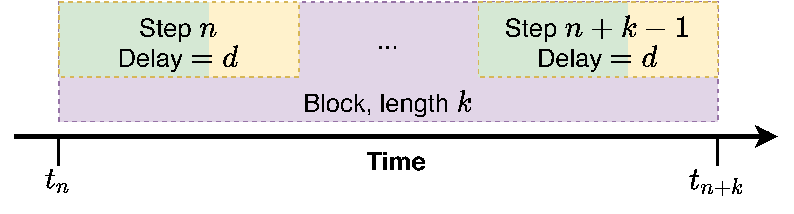
\includegraphics[width=.6\textwidth]{publications/2021ImpactDelayedResponse/Fig4c}
    \caption{Structure of a \emph{block} in the experimental LEGO task.}\label{fig:stepblock}
    \todo[inline]{This figure may need reworking for clarity.}
\end{figure}

The actual \gls{WCA} task employed for this study corresponded to a modified and extended version of the LEGO assembly task introduced in~\cite{chen2015early}.
Unlike the original design of this task, in which the user is led through the assembly of a specific model, the modified LEGO task consisted of a pseudo-random sequence of steps instructing subjects to add or remove pieces.

We introduced an experimental design component denoted a \emph{block}, illustrated in \cref{fig:stepblock}, corresponding to a segment of consecutive steps subject to the same delay value.
To study the effects of a delay applied across multiple steps, we manipulated the length of blocks during the task, using values of \numlist[list-final-separator={, or }]{4;8;12} steps.
Furthermore, we defined a \emph{slice} as a continuous segment of \num{4} steps within a block.
In other words, \num{4}-step blocks were composed of a single slice, whereas \num{8}- and \num{12}-step blocks were composed respectively of \num{2} and \num{3} consecutive slices.

Using the above experimental design components, we then generated a task for each participant.
We generated a pseudo-random permutation of the combinations of block length and delay values, and assigned a unique sequence of steps to each combination in order to create \num{21} unique blocks of steps.
Using a \emph{Latin-square}~\cite{keedwell2015latin} design, we reordered the initial permutation to generate \num{40} tasks.

To measure the extent to which individual differences in each subject affected obtained task-performance results, participants were asked to complete two questionnaires previous to beginning the task;
the \gls{BFI}~\cite{john1999big} and the \gls{ITQ}~\cite{witmer1998measuring}.
These correspond to well-established tools for the measurement of individual personality traits in humans.
The \gls{BFI}~\cite{john1999big} consists of \num{44} questions assessing the traits of
\begin{enumerate*}[itemjoin={{, }}, itemjoin*={{, and }}]
    \item agreeableness
    \item conscientiousness
    \item extroversion
    \item neuroticism
    \item openness
\end{enumerate*}.
The \gls{ITQ}~\cite{witmer1998measuring}, on the other hand, assesses involvement, focus, and the tendency to play games, using \num{29} questions.
The scores for these questionnaires were normalized in post-processing to fall in the \ensuremath{[0, 1]} range for ease of interpretation.

In order to try to capture metrics relating to the emotional response of humans to changes in system responsiveness, participants were asked to wear an array of biometric sensors.
This array included devices to capture four physiological measures:
\begin{enumerate*}
    [itemjoin={{, }}, itemjoin*={{, and }}, label={(\arabic*)}]
    \item \gls{GSR} (also known as electrodermal activity)
    \item accelerometer data from the dominant wrist
    \item brain activity in the form of \gls{EEG}
    \item heart rate
\end{enumerate*}.
Unfortunately, no statistically significant effects were measured in any of these variables, and as such neither will be discussed in this summary.
Please refer to \cref{paper:olguinmunoz2021impact} for details.

Finally, we collected video recordings of participants' faces and as well as of the live feed of frames provided as input to the \gls{WCA}.
The facial recordings will also not be discussed in this section, as they were not employed in any analyses.
However, the recording of the live feed was employed later on in the implementation of a procedure for the generation of dynamic synthetic traces for the LEGO task in the context of the EdgeDroid load generator for \gls{WCA}.
This will be discussed in \cref{model:traces}.

\subsubsection{Results}\label{impact:results}

\begin{figure*}[tb]
    \centering
    \begin{subfigure}[t]{0.45\textwidth}
        \includegraphics[height=13em]{./Figs/2021Impact/ttf_vs_exectime_per_block}
        \caption{%
            \gls{TTF} vs average execution time, grouped by block length.
            Transparent bands indicate \SI{95}{\percent} \glspl{CI}.
        }\label{fig:ttfvsexectime:block}
    \end{subfigure}%
    \hfill%
    \begin{subfigure}[t]{0.45\textwidth}
        \includegraphics[height=13em]{./Figs/2021Impact/ttf_vs_exectime_per_slice}
        \caption{%
            \gls{TTF} vs average execution time, grouped by step slice in a block.
            Slice \num{1} corresponds to steps \numrange{1}{4}, \num{2} to steps \numrange{5}{8}, and \num{3} to steps \numrange{9}{12} in a block.
            Blocks with \num{4} steps only contribute to slice \num{1}, and blocks with \num{8} steps to slices \num{1} and \num{2}.
            Transparent bands indicate \SI{95}{\percent} \glspl{CI}.
        }\label{fig:ttfvsexectime:slice}
    \end{subfigure}%
    \caption{Effects of perceived \gls{TTF} on measured step execution times by participants.}\label{fig:ttfvsexectime}
\end{figure*}

\Cref{fig:ttfvsexectime} shows effects on the measured execution times of participants as perceived \gls{TTF} increased.
These results have been grouped by block length (\cref{fig:ttfvsexectime:block}), showing the cumulative effects of delay over series of steps, and slice number (\cref{fig:ttfvsexectime:slice}), showing the evolution of these effects within a series of steps at the same level of impairment.

\cref{fig:ttfvsexectime:block} shows that as system responsiveness decreased, the speed at which participants completed instructions tended to slow down.
Compared to the unimpaired case, participants were on average \SI{12}{\percent} slower when subject to a mean \gls{TTF} of \SI{2.475}{\second}, and \num{26} percentage points slower at a mean \gls{TTF} of \SI{4.5}{\second}.
\Cref{fig:ttfvsexectime:block} illustrates this effect clearly;
for all block lengths, as \gls{TTF} grows we see an accompanying increase in execution times.
Moreover, this effect seemed stronger for longer blocks at higher levels of impairment, indicating a slow-down which compounds with the number of steps.
Note that by measuring \emph{step execution time} we are \emph{per se} compensating for the added delay in the measure, and thus this trend must result from the participants' behavioral slow-down as a response to the perceived increase in \gls{TTF}.
This was confirmed through an \gls{ANOVA}~\cite{fujikoshi1993two} including factors of block length and \gls{TTF}; significant effects were found for both factors and their interaction (\ensuremath{p < 0.01}).

On the other hand, in \cref{fig:ttfvsexectime:slice} we observe the evolution of execution times over \emph{slices} of \num{4} steps within blocks.
This figure illustrates how, at the lowest levels of impairment, users tended to get faster as the task progressed.
At the lowest \gls{TTF}, the average execution time of steps \num{9} to \num{12} in a block was roughly \textasciitilde\SI{26}{\percent} lower than for steps \num{1} to \num{4}.
However, this effect is strongly dampened at higher levels of impairment, with the difference between the average execution times of steps in slices \num{2} and \num{3} basically disappearing at the highest \gls{TTF}.
This was also confirmed through an \gls{ANOVA} on factors slice and \gls{TTF}, finding significant (\ensuremath{p < 0.01}) for both factors and their interaction.

\begin{figure}
    \begin{minipage}[t]{.45\textwidth}
        \centering
        \includegraphics[height=13em]{Figs/2021Impact/previousblock_vs_exectime}
        \caption{Mean execution time of the first slice of steps in a block, grouped by \glsfmtshort{TTF} of the block immediately preceding the current one.}\label{fig:prevblockvsexectime}
    \end{minipage}%
    \hfill%
    \begin{minipage}[t]{.45\textwidth}
        \centering
        \includegraphics[height=13em]{publications/2023EdgeDroid2/figs/new_model/mu_fits_exgaussian_slice0}
        \caption{%
            Illustration of the effect of neuroticism on the \ensuremath{\mu} parameter of \glsfmtshort{exGaussian} distributions fitted to the execution times of steps in slice \num{1}.
            Fits were achieved through \gls{MLE}.
        }\label{fig:ttfvsexgaussianmu}
    \end{minipage}
\end{figure}

As mentioned before, we found that the effects of system responsiveness on execution times lingered on after the system moved to a different level of impairment.
\Cref{fig:prevblockvsexectime} illustrates this effect.
On average, the mean execution time of the first four steps of blocks was roughly \SI{7}{\percent} lower when the previous block was at a \ensuremath{TTF \leq \SI{2.475}{\second}} compared to when the previous block was at a \ensuremath{TTF > \SI{2.475}{\second}} (single-tailed \ensuremath{p < 0.001}).

Analyses of the correlation between individual subject differences and the above effects highlighted the \gls{BFI} trait of \emph{neuroticism} as an important modulating factor.
This trait has been linked to low tolerance for stress, high emotional reactivity, as well as higher rates of \emph{delay discounting}~\cite{hirsh2008delay}.
Out of the three components identified by a \gls{PCA}, which cumulatively accounted for \textasciitilde\SI{73}{\percent} of the variance in the execution time results, neuroticism was present in the first two.
Individual neuroticism scores were found to significantly linearly correlate (\ensuremath{rho = 0.418}, two-tailed \ensuremath{p < 0.05}) with measured execution times at high \glspl{TTF}.

Finally, we found that execution times were well-fit by \gls{exGaussian} distributions.
Previous research has established strong arguments for the use of this distribution for the modeling of human reaction times and the timings of human actions~\cite{rohrer1994analysis,palmer2011what,marmolejo_ramos2022generalised}.
When grouping execution times by low/high neuroticism\footnote{%
    \emph{Low} refers to values less than the middle value obtainable for neuroticism in the \gls{BFI}; \emph{high} to values greater than or equal to it.
}, \gls{TTF}, and slice, the best fit statistic obtained using a Kolmogorov-Smirnov goodness-of-fit test~\cite{massey_jr1951kolmogorov} was \num{0.028}, with a \ensuremath{p}-value of \num{0.999}.
The effects of neuroticism were most easily observed in the \ensuremath{\mu} parameter and the tails of the fitted distribution;
an example of this can be observed in \cref{fig:ttfvsexgaussianmu}.
There is a clear and direct correlation between higher neuroticism and higher \ensuremath{\mu} values and longer tails.

\subsubsection{Implications}

The results summarized above lead to interesting implications for the design and optimization of \gls{WCA} application systems.
The behavioral slow-down in users as a response to reductions in system responsiveness translates into noticeably extended application lifetimes, even for short durations of impairment.
Combined with the permanence of these effects for a period even after the system returns to an improved level of responsiveness, this could lead to unconventional consequences for resource allocation, in particular in multi-tenant deployment and in cases where a user may be able to finish the task before the effects of slow-down subside.
In such cases, it might be more efficient to not divert resources to the impaired application, as fair degradation may not ultimately be beneficial to the system as a whole.
It might even be more beneficial to divert resources \emph{away} from the impaired application, to ensure optimal system responsiveness for other tenants in the system.

These implications, however, are merely speculative.
Moreover and as previously discussed, due to the complexity of these systems, accurate study of the actual consequences of the results discussed in the present section can only be achieved through an experimental approach.
\todo[inline]{Does this need a better transition?}


\subsection{A new model of human behavior in \glsfmtshort{WCA}}

\cref{paper:olguinmunoz2023realistic} discusses the elaboration of a model of human behavior for \gls{WCA}.
Built upon the data and results from \cref{paper:olguinmunoz2021impact}, our model is capable of dynamically generating realistic predictions of execution times for steps in a \gls{WCA} based on historical system state data and a parameterized level of neuroticism.
Furthermore, we implement a new version of the EdgeDroid tool capable of using this new model, together with a novel procedure for the generation of realistic synthetic traces of frames for \gls{WCA}, to fully emulate a human in the context of these systems.

\subsubsection{Design of a realistic model for human timings in \gls{WCA}}

\todo[inline]{Probably needs to repeat a discussion on why the new model is necessary, in a shorter summarized form.
This discussion should first be presented at the beginning of this section however.}

As discussed in \cref{impact:results}, the execution time for a step depends not only on the most recent perceived \gls{TTF}, but also on how long the system has been in the current level of responsiveness.
Moreover, as shown in \cref{fig:prevblockvsexectime}, the effects of reduced system responsiveness on generated execution times must be taken into consideration even after the system transitions into a more responsive state.
All of these effects are also modulated by neuroticism, adding both another layer of complexity and a means of parameterizing the model.

Our timing model produces realistic execution times for each step, according to the above effects.
We achieve this through the following design:

\begin{enumerate}
    \item Our model takes two inputs, the measured \gls{TTF} for the most recent step and a level of normalized neuroticism.
    We use two levels of neuroticism: \emph{low}, for normalized values in the range \ensuremath{[0, 0.5)}; and \emph{high}, for the range \ensuremath{[0.5, 1.0]}.
    \item The model is stateful, keeping the values of the \num{12} most recent \glspl{TTF} in memory.
    \item Whenever a new \gls{TTF} is received, the thirteenth most recent \gls{TTF} is dropped, and a weighted average is calculated using the values in memory.
    This value is obtained using the formula
    \begin{equation}
        \label{eq:modelweights}
        w_{n - i} =
        \left\{ \begin{array}{ll}
                    \frac{e^{-0.7 i}}{\sum\limits^{12}_{j=1} e^{-0.7 j}} & 1 \leq i \leq 12 \\
                    &                  \\
                    0                                                    & i > 12
        \end{array} \right.
    \end{equation}
    This results in the \gls{TTF} for the most recent step accounting for approximately \SI{50}{\percent} of the weighted result, with this percentage decaying by a factor of about \ensuremath{\frac{1}{2}} for each step further back in the sequence.

    \item The resulting weighted rolling \gls{TTF} is used to look up potential values for the execution time in the original data from \cref{paper:olguinmunoz2021impact}.
    We do this by pre-processing the original data from the \num{40} independent repetitions of the LEGO task with this same rolling weighted average formula, and then binning samples according to the resulting \num{7}-quantiles for weighted \glspl{TTF}.
    The weighted \gls{TTF} calculated during runtime is then matched to the corresponding bin of samples.

    \item The selected samples are further filtered according to the selected level of neuroticism for the model.
    \item Finally, a realistic execution time for the step is generated either by directly sampling the execution time values from the selected samples, or first fitting a theoretical \gls{exGaussian} distribution to these values and then sampling the distribution instead.
\end{enumerate}

\begin{figure}[tb]
    \centering
    \includegraphics[width=\textwidth]{Figs/2023EdgeDroid2/model_exectime_over_steps}
    \caption{
        Illustration of the execution times output by the model at fixed values of \glspl{TTF}, over a series of steps, parameterized by levels of neuroticism.
        Shaded bands indicate \SI{95}{\percent} \glspl{CI}.
    }\label{fig:model:exectimesoversteps}
\end{figure}

\begin{figure}
    \begin{minipage}[t]{.45\textwidth}
        \centering
        \includegraphics[width=\textwidth]{Figs/2023EdgeDroid2/model_exectimes_transition}
        \caption{%
            Mean execution times generated by the model after a single step at a \gls{TTF} of \SI{2.5}{\second} preceded by a sequence of \num{25} steps at fixed lower (instantaneous feedback) or higher (\SI{5}{\second}) \gls{TTF}.
            Errorbars indicate \SI{95}{\percent} \glspl{CI}.
        }\label{fig:model:exectimestransitions}
    \end{minipage}%
    \hfill%
    \begin{minipage}[t]{.45\textwidth}
        \centering
        \includegraphics[width=\textwidth]{publications/2023EdgeDroid2/model_data/frame_probabilities}
        \caption{%
            Distribution of processing results for frames captured during the execution of steps in the LEGO task.
            Note that \emph{Success} results are not included since by definition \ensuremath{P(\text{Success}|t_\text{norm}) = 1.0} for all normalized instants \ensuremath{t_\text{norm} \geq 1.0}.
        }\label{fig:modelframes}
    \end{minipage}
\end{figure}


\Cref{fig:model:exectimesoversteps,fig:model:exectimestransitions} illustrate the adherence of the model to the conclusions obtained from our work in \cref{paper:olguinmunoz2021impact}.

\Cref{fig:model:exectimesoversteps} shows the output of the execution time model described above over a series of steps at three levels of \gls{TTF};
\emph{low} (instantaneous feedback), \emph{medium} (\SI{2.5}{\second}), and \emph{high} (\SI{5}{\second}).
When the system is highly responsive (low \glspl{TTF}), the model tends to speed up as the task progresses.
Conversely, at high levels of impairment, execution times depend on strongly on the parameterized level of neuroticism;
as concluded from our previous discussion, higher neuroticism leads to a stronger reaction to reduced responsiveness and subsequently to longer execution times.

In \cref{fig:model:exectimestransitions}, moreover, we present the lingering effects of reduced system responsiveness on \glspl{TTF} generated after the system returns to a more responsive state.
These results were generated by first feeding a sequence of \num{25} identical \glspl{TTF} to the model, with values of either \SI{0}{\second} (i.e.\ instantaneous feedback) or \SI{5}{\second}.
Next, a single \gls{TTF} of \SI{2.5}{\second} was fed to the model, and the generated execution time was recorded.
This procedure was repeated \num{600} times.
As expected from our discussion in \cref{impact:results}, transitions from a higher (\SI{5}{\second}) \gls{TTF} resulted in noticeably inflated execution times (\ensuremath{+\SI{8.5}{\percent}} at a high level of neuroticism) for the first step at \SI{2.5}{\second} \gls{TTF} compared to when the transition was from a lower \gls{TTF}.

\subsubsection{Procedural generation of dynamic traces of video frames for \glsfmtshort{WCA}}\label{model:traces}

Our design for a procedure for the generation of synthetic yet realistic traces of video inputs for \gls{WCA} follows a stochastic approach.
Analysis of the evolution of the distribution of processing results of frames over their normalized capture instant with respect to step execution time highlighted the pattern illustrated in \cref{fig:modelframes}.
We define the normalized capture instant \ensuremath{t_\text{norm}} for each frame as the timestamp at which it was captured with respect to the beginning of the step, normalized by the total execution time of the same step.
The distribution of the four possible categories of outputs of the \gls{CV} algorithm in the Gabriel LEGO Task~\cite{chen2018application} for each frame (\emph{blank}, i.e.\ no discernible board state, noise; \emph{low confidence}; \emph{success}, a frame which triggers a step transition;
and \emph{repeat}, that is, no change since the last \emph{success} frame) were plotted against normalized capture instants.

These results are then used together with a repository of tagged frames for each step to generate a synthetic trace at runtime by:
\begin{enumerate}
    \item At each sampling instant, calculate the current \ensuremath{t_\text{norm}} with respect to the next desired execution time.
    \item If \ensuremath{t_\text{norm} \geq 1}, send a pre-selected \emph{success}-tagged frame for the current step to the \gls{WCA} backend.
    \item Otherwise, sample the distribution of result categories at the selected \ensuremath{t_\text{norm}} and return a pre-selected frame matching the selected category.
\end{enumerate}

This procedure results in a synthetic stream of frames which generates the same processing load on the backend as a real stream would.
The use of a repository of frames collected from real executions of the task by humans ensures that the load on the network also approximates reality.
More details and a longer discussion on this approach can be found in \cref{paper:olguinmunoz2023realistic}, \cref{ssec:model:frames}.

\subsection{Implications with respect to task completion times}

In this section, we will discuss the implications of the methodology for the optimization of \gls{WCA} applications, in particular when employing the experimental results and the improved model of human timings discussed in \cref{sec:extendingmethodology}.
The discussion presented here is a summarized version of what \cref{paper:olguinmunoz2023realistic} exposes.

\todo[inline]{Do we need more experiments?}
\todo[inline]{Include discussions on the metrics here (grab inspiration from EdgeDroid2 paper.)}


The term \emph{task completion time}, in the context of \gls{WCA}, will refer to the time it takes a user to work their way through the task presented by an assistant application.
In \cref{paper:olguinmunoz2023realistic} we refer interchangeably to task completion times as application lifetimes.
This metric directly relates to system resource and energy consumption --- longer task completion times mean that the system is occupied for longer and thus uses more resources.
It thus presents a relatively straightforward yet interesting starting point for the study of the implications of the model on the optimization of \gls{WCA} systems.

\begin{figure}
    \centering
    \includegraphics[height=13em]{Figs/2023EdgeDroid2/task_durations_diff}
    \caption{Difference in task completion times of the realistic model with respect to the reference baseline.
    Geometric averages over \num{10} over ten total repetitions per configuration.}\label{fig:taskcompletiontimesdiff}
\end{figure}

The main question we aim to ask relates to the consequences of using our model of human timing behaviors versus using a less realistic approximation.
Specifically, we aim to quantify the difference in task completion times when using the realistic model compared to a baseline which does not take into consideration higher order effects on execution times.
In \cref{fig:taskcompletiontimesdiff} we present the results of an experimental exploration of this difference.
We compare the total task durations of emulated \num{45}-step tasks using the EdgeDroid benchmarking tool with the improved model of human behavior to a baseline model.
Our reference baseline corresponds here to a first order approximation to empirical execution time modeling, using an \gls{exGaussian} distribution fitted to \emph{all} the data points from \cref{paper:olguinmunoz2021impact} (without any grouping) which is randomly sampled to obtain execution time values.
We perform this experiment on the edge computing testbed discussed in \cref{sec:testbed};
for simplicity and to magnify the effects of latency, in this setup we use an \glsfmtshort{IEEE} \num{802.11}b/g physical layer.

These results show clear and significant differences in task durations between the realistic model and the baseline, with a reduction of up to \SI{11}{\percent} at low levels of resource contention for both levels of neuroticism.
At higher degrees of resource contention, the high neuroticism parameterization also results in task durations more than \SI{8}{\percent} longer than the baseline.

\todo[inline]{Briefly discuss implications of the above?}

\subsection{Implications with respect to number of samples per step}

In the present section and the following we briefly discuss the implications of our methodology on the optimization potential of number of samples and energy consumption per step, respectively.
Both these analyses depend on an understanding of the tradeoffs between resource consumption and responsiveness in \gls{WCA};
fewer samples per step translates into longer sampling periods, and lower energy consumption tends to be made possible by processing fewer bits of data per step.
As such, we employ in these sections an optimization framework for the optimization of said trade-offs based primarily upon the work of Moothedath et al.~\cite{moothedath2021energy,moothedath2022energy1,moothedath2022energy2}.
We note that objective metrics relating to sampling and the responsiveness of a \gls{WCA} system will present itself as a linear combination of the number of expected samples and expected wait time per step plus some constant term:
\begin{align}
    \mathcal{E} = \alpha\mathbb{E}[\mathcal{S}] + \beta\mathbb{E}[\mathcal{W}] + C\label{eq:genericopt}
\end{align}
The above objective function is generic, and can be adapted to any metric which relates to the sampling and responsiveness of \gls{WCA} by modifying the factors \ensuremath{\alpha}, \ensuremath{\beta}, and \ensuremath{C}.

For the analyses in this subsection and \cref{ssec:implications:energy}, we use the solution
\begin{align}
    t_n = \left( 3\sigma\sqrt {\frac{\alpha}{2\beta}} \right)^{\frac{2}{3}} n^{\frac{2}{3}}
\end{align}
where \ensuremath{t_n} once again corresponds to the \ensuremath{n}-th sampling instant in a step.
Note that any positive real value is valid for \ensuremath{\frac{\alpha}{2\beta}}.
This ratio controls the optimization criteria --- as it goes to infinity, the criteria changes from minimizing wait time (i.e.\ maximizing responsiveness) to minimizing the number of samples per step (i.e.\ minimizing energy consumption).

The full derivation and explanation of this framework is out of the scope of this summary.
Please refer to \cref{paper:olguinmunoz2023realistic} and its appendix for a detailed discussion on this optimization approach.
\todo{Include ref to section?}

\medskip





\subsection{Implications with respect to raw energy consumption}\label{ssec:implications:energy}
